%3.1. pi-SoD-M metamodels (presentar los metamodels)


The {\em A-policy} based service composition ($\pi$-SCM) meta-model, described in Figure \ref{fig:e-scomposition-metamodel},
provides classes to represent workflows\footnote{Workflows will be transformed into implemented service compositions.}.
The meta-model identifies {\sc Business Collaborators}\footnote{We use {\sc capitals} for referring to meta-model classes.} and the {\sc Actions} they perform. 
Instances of this meta-model are UML activity diagrams. 
Figure~\ref{fig:e-scomposition-metamodel} show the modelling elements.
Classes pictured as coloured boxes deal with non-functional properties.
The classes pictured with a white background are those of SOD-M.

In the meta-model of Figure~\ref{fig:e-scomposition-metamodel}:
\begin{itemizedTrivlist}
\item A {\sc Business Collaborator} element represents those entities that collaborate in the business processes by performing some of the required actions. 
They are graphically presented as a partition in the activity diagram. 
A collaborator can be either internal or external to the system. 
When the collaborator of the business is external to the system, the attribute {\sf IsExternal}\footnote{We use the {\sf sans serif} font for referring to classes defined using a meta-model.} of the collaborator is set to \textbf{true}.

\item {\sc Action}s, a kind of {\sc ExecutableNode}, are represented in the model as an activity. 
Each action represents some type of transformation or processing. 
There are two types of actions: i) a WebService (attribute Type is {\sf WS}); and ii) a simple operation that is not supported by a Web Service, called an {\sc ActivityOperation} (attribute Type is {\sc AOP}).
\begin{figure}[t]
\centering
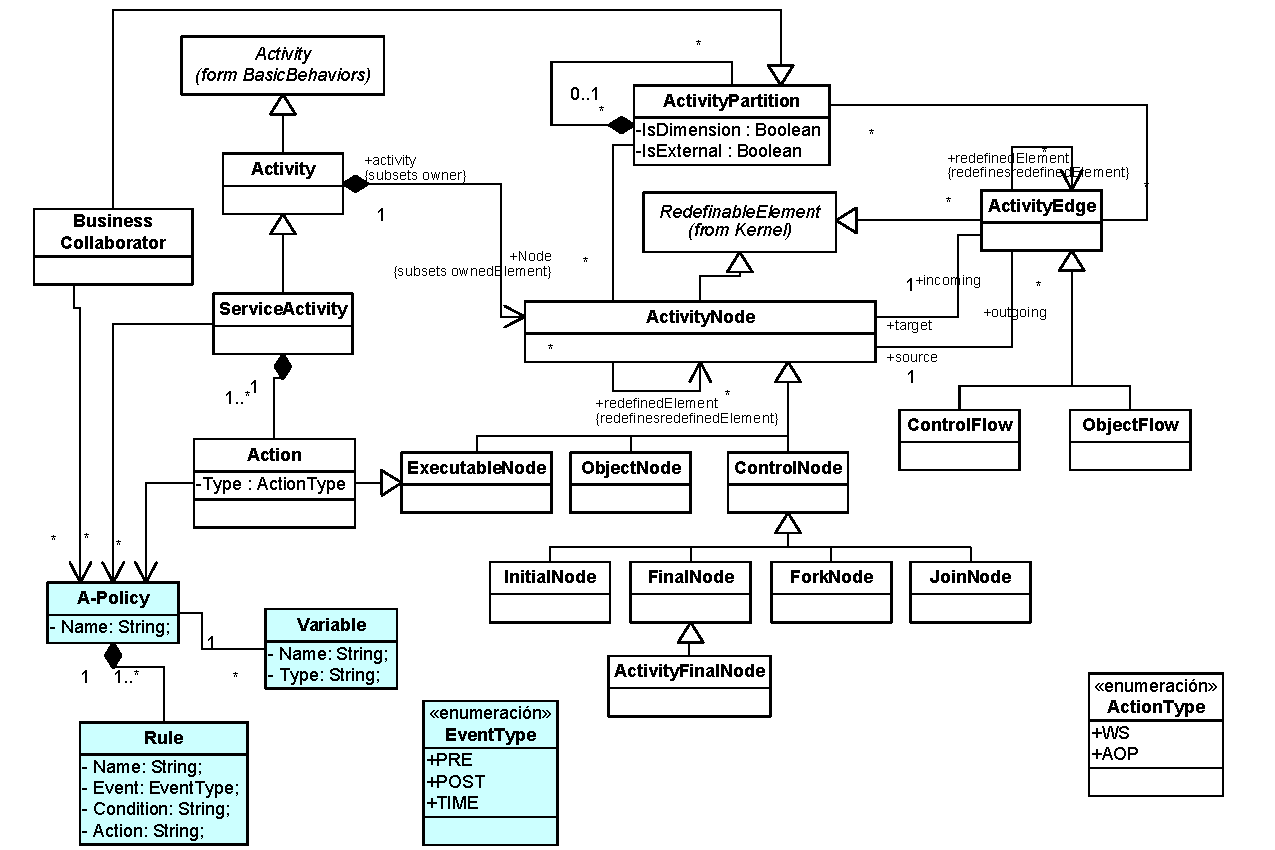
\includegraphics[width=1.0\textwidth]{figs/E-service-composition-metamodel}
\caption{$\pi$-Service Composition ($\pi$-SCM) Metamodel.}
\label{fig:e-scomposition-metamodel}
\end{figure}

\item The {\sc ServiceActivity} element is a composite activity that must be carried out as part of a business service and is composed by one or more executable nodes.

\item In order to represent constraints associated to services compositions, we extended the SOD-M service composition model with two concepts: {\sc Rule} and {\sc A-policy} (see blue elements in the $\pi$-SCM meta-model in Figure \ref{fig:e-scomposition-metamodel}).
We model non-functional constraints by using the notion of {\em A-policy}~\cite{Espinosa-Oviedo2011a,CIC:eovszmc09c}.
An {\em A-policy} is formed by attributes and rules. 
Intuitively, the conditions of each rule will be checked.
In case of no compliance, the actions defined by the rule will be performed.
The {\sc Rule} element represents an event - condition - action rule where the {\sc Event} part represents the moment in which a constraint  will be evaluated.
An {\em A-policy} defines variables and operations that can be shared by the rules and that can be used for expressing their Event and Condition parts. 
\end{itemizedTrivlist}

\begin{figure}[t]%[htpb]
\centering
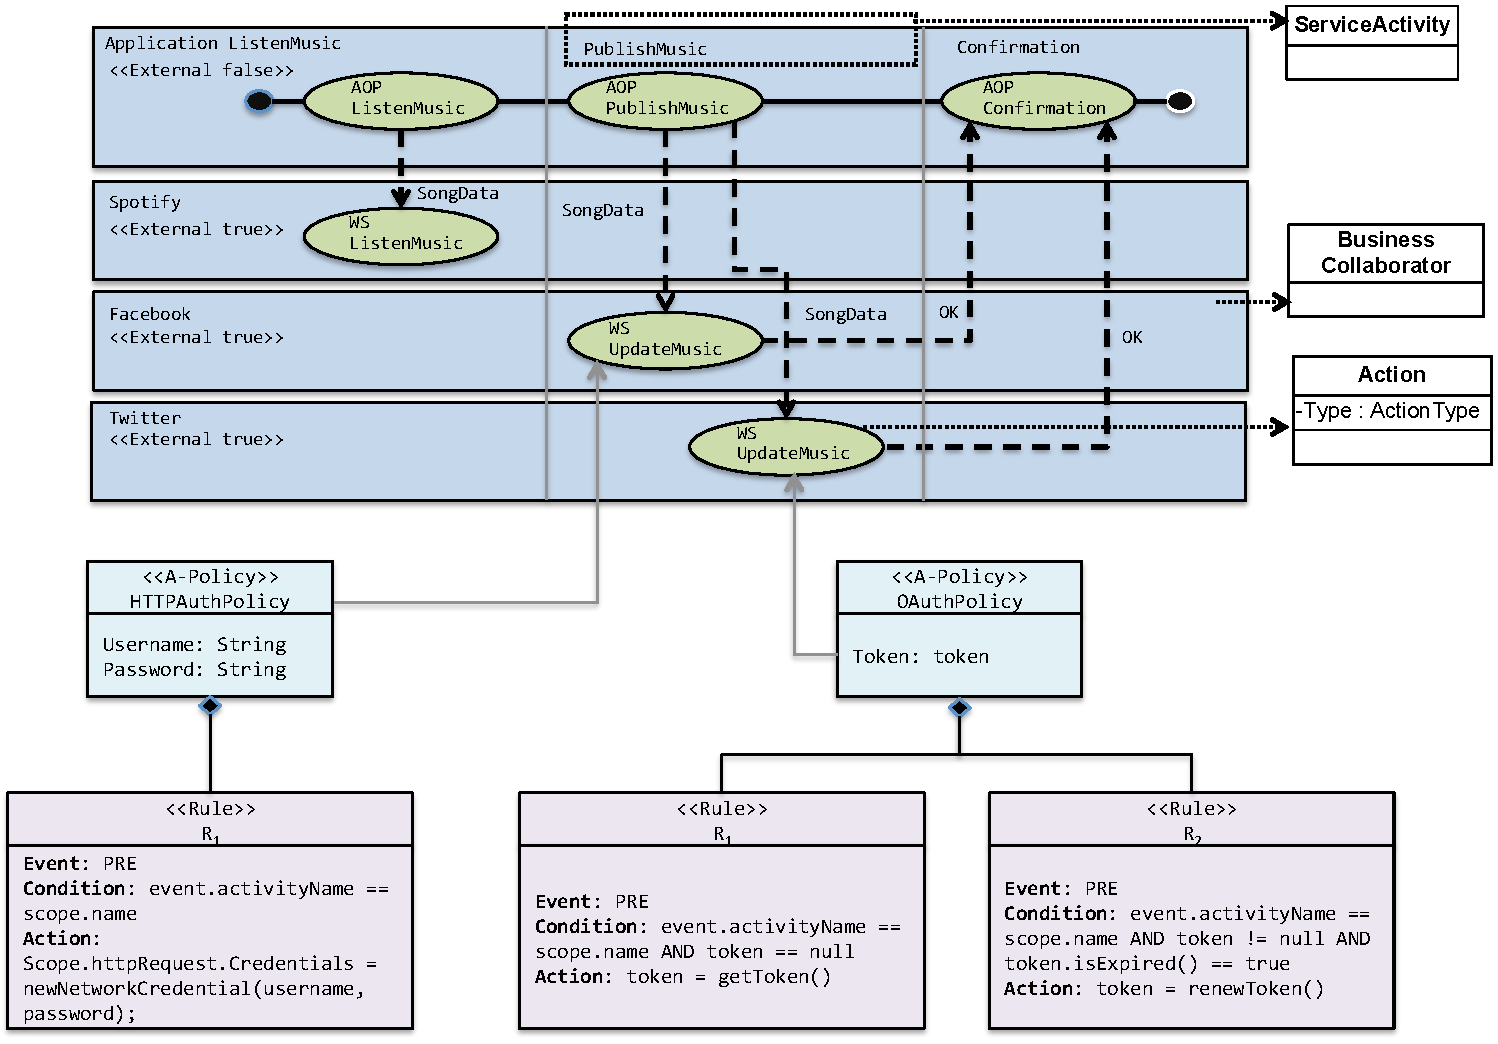
\includegraphics[width=0.95\textwidth]{figs/e-composition-model}

{\color{red}\LARGE PLACIDO: Please change the names of the boxes in accordance to the explanation --Martin}

\caption{$\pi$-SCM for the ``To publish music'' business service.}
\label{fig:servicecompositionmodel}
\end{figure}

\begin{example}[To Publish Music]\label{ex:toPublicMusic}
To illustrate the use of the $\pi$-Service Composition Meta-model, we define a model for the ``To Publish Music'' scenario (Figure \ref{fig:servicecompositionmodel}). 
In this model, there are three external business collaborators ({\em Spotify, Twitter} and {\em Facebook}).
% \footnote{We use {\em italics} to refer to concrete values of the classes of a model that are derived from the classes of a meta-model.}). 
The model also shows the business process of the application that consists of three service activities: {\em Listen Music}, {\em Public Music} and {\em Confirmation}. 
Note that  the activity {\em Publish Music} calls the actions of two service collaborators namely {\em Facebook} and {\em Twitter}.
Both {\em Facebook} and {\em Twitter} services require authentication protocols in order to execute methods that will read and update the user space. 
%A call to such services must be part of the authentication protocol required by these services.
In the example we  associate two authentication policies, one for the open authentication protocol, represented by the class {\sf\small OAuthPolicy} at {\em Twitter}, that will be associated to the activity  {\sf\small UpdateTwitter} (see Figure \ref{fig:servicecompositionmodel}). 
In the same way, the {\em Facebook} class {\sf\small HTTPAuthPolicy}, for the http authentication protocol will be associated to the activity {\sf\small UpdateFacebook}.

{\sf\small OAuthPolicy} will implement the open authentication protocol.
The {\em A-policy} {\sf\small OAuthPolicy} has a variable {\sf\small Token} that will be used to store the authentication token provided by the service.
This variable is imported through the library {\sf\small OAuthPolicy.Token}. 
The A-policy {\sf\small OAuthPolicy} defines two rules, both can be triggered by events of type {\sf\small ActivityPrepared}: (R$_1$): If no token has been associated to the variable {\sf\small token}, then a token is obtained ; and (R$_2$): if the token has expired, then it is renewed. 
Notice that the code in the actions profits from the imported {\sf\small OAuthPolicy.Token} for transparently obtaining or renewing a token from a third party.

{\sf\small HTTPAuthPolicy} implements the HTTP-Auth protocol. 
The A-policy imports an http protocol library and it has two variables {\sf\small username} and {\sf\small password}.  
The event of type {\sf\small ActivityPrepared} is the triggering event of the rule {\sf\small R$_1$}. 
On the notification of an event of that type, a credential is obtained using the username and password. 
\hfill\openbox
\end{example}

We propose the use of rules and policies to model and associate non-functional properties to service compositions.
These artifacts will be used to generate the actual programs that will implement the application:
Once the $\pi$-Service Composition Model has been defined, then it can be transformed into a lower level model (in our case, $\pi$-PEWS) that gives support to code generation. 
The $\pi$-PEWS  meta-model is described in the next section. 


%..--..--..--..--..--..--..--..--..--..--..--..--..--..--..--..--..--..--..--..--..--..--..--..--..--..--..--..--..--..--..--..
\subsubsection{$\pi$-{\sc Pews}  meta-model}\label{sec:pewsmetamodel}
%..--..--..--..--..--..--..--..--..--..--..--..--..--..--..--..--..--..--..--..--..--..--..--..--..--..--..--..--..--..--..--..

PEWS~\cite{BHM06,Placido2010LTPD} is a notation to express service compositions.
The language is based on the notion of Path Expressions~\cite{And79} and can easily be translated into any actual composition language, such as B	PEL~\cite{bpel03} or any other language that lets the service designer combine the methods or subprograms that implement each operation of a service, in order to achieve the desired application logic. 
Figure~\ref{fig:metamodel} presents the $\pi$-{\sc Pews} meta-model, where we identify classes to describe:
\begin{itemizedTrivlist}
\item Service compositions: {\sc Namespace} representing the interface exported by a service, {\sc Operation} that represents a call to a service method, {\sc CompositeOperation}, {\sc Operator} and {\sc Path} for representing service compositions.
A {\sc Path} can be an {\sc Operation} or a {\sc Compound Operation}. 
A {\sc Compound Operation} is defined using an {\sc Operator}.
The language defines operators to denote guarded operations ($[C]S$); sequential ($\ . \ $), parallel ($\ \| \ $) and alternative ($\ + \ $) compositions; as well as sequential ($*$) and parallel ($\{\dots\}$) repetition.

\item {\em A-Policies} that can be associated to a service compositions:  {\sc A-Policy}, {\sc Rule}, {\sc Event}, {\sc Condition}, {\sc Action}, {\sc State}, and {\sc Scope}.
A brie description of these classes is given next.
\end{itemizedTrivlist}
%
\begin{figure}[t]
\centering
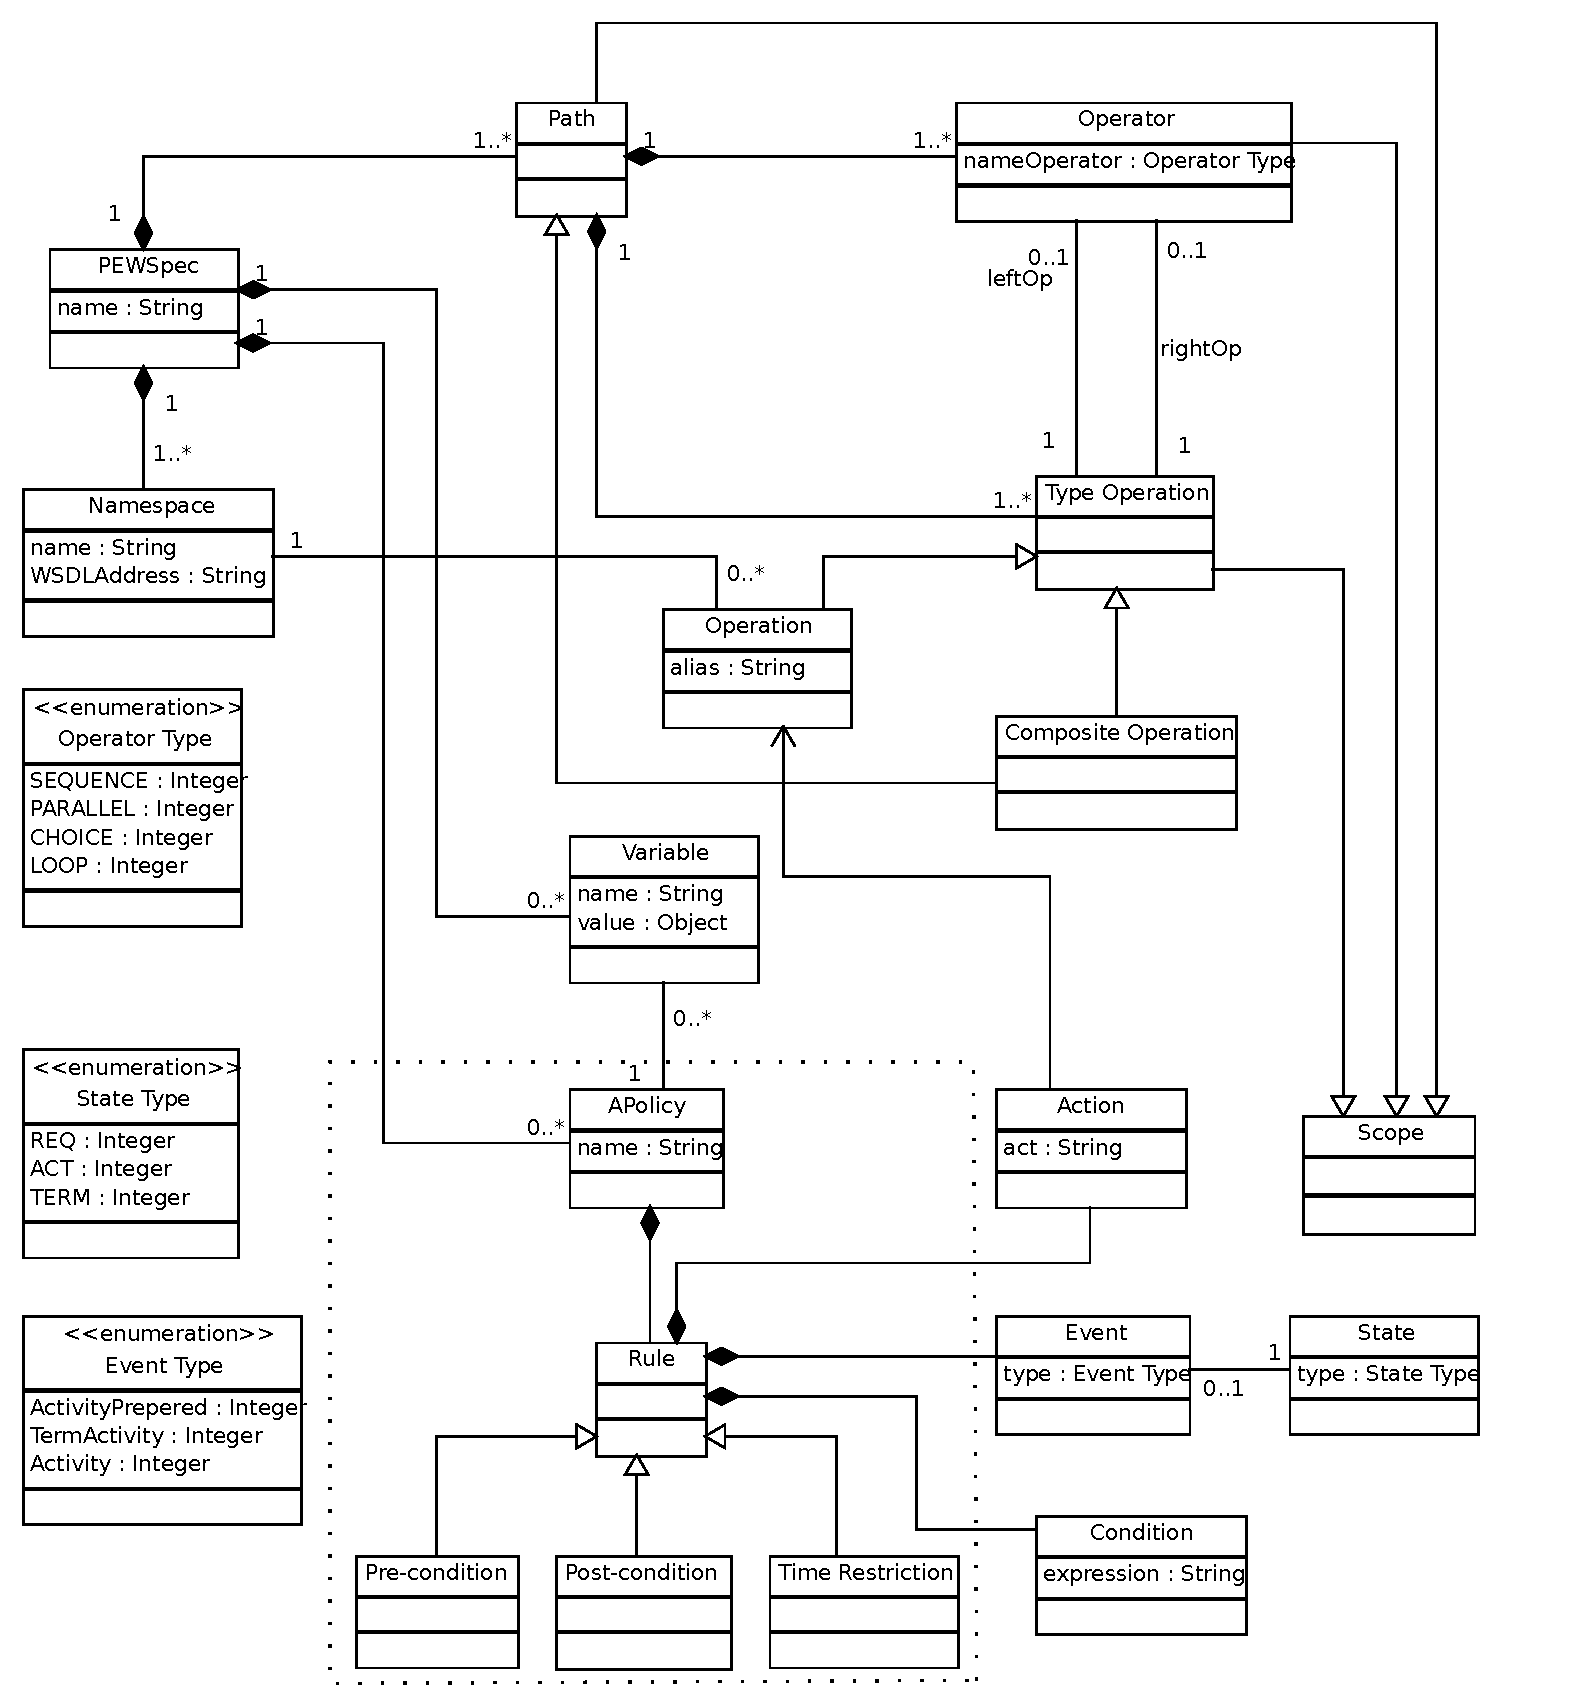
\includegraphics[width=1.0\textwidth]{figs/PEWSMetamodel}
\caption{$\pi$-{\sc Pews} Metamodel}
\label{fig:metamodel}
\end{figure}

Figure~\ref{fig:metamodel} shows that each {\sc A-Policy} is associated to a {\sc Scope} that can be either an {\sc Operation} (e.g., an authentication protocol associated to a method exported by a service),  an {\sc Operator} (e.g., a temporal constraint associated to a sequence of operators) or a {\sc Path}.  
Each {\sc A-Policy} groups a set of ECA rules with a classic semantics, i.e, {\em when an event of type E occurs, if condition C is verified then execute the action A}.  
In this way, an {\em A-policy} represents a set of reactions to be possibly executed when one or several events are notified.
%In this way,
%\begin{itemizedTrivlist}
%\item The class {\sc Scope} represents any element of a service composition (i.e., operation, operator, path).
%\item The class {\sc A-Policy} represents a recovery strategy implemented by ECA rules of the form {\sc Event} - {\sc Condition} - {\sc Action}. 
%An {\em A-policy} has variables that represent the view of the execution state of its associated scope, that is required for executing the rules. The value of a variable is represented using the type {\sc Variable}. The class {\sc A-Policy} is specialized for defining specific constraints, for instance authentication {\em A-policies}.
%\end{itemizedTrivlist}
%
%An authentication {\em A-policy} represents the situation where an invocation in
%an activity occurs until its sender and/or its recipient have been
%identified. Typically, authentication A-Policies ensure that the invocation of the activity will be done within an authentication protocol.

Given a $\pi$-SCM model of a specific service based application (expressed according to the $\pi$-SCM meta-model), it is possible to generate its corresponding $\pi$-{\sc Pews} model. 
The following section describes the transformation rules between the $\pi$-SCM and $\pi$-{\sc Pews} meta-models.



